\documentclass{beamer}
\usepackage[utf8]{inputenc}
\usepackage[slovene,english]{babel}

\usetheme{default}

\title{Vrtače dinarskega krasa}

% A subtitle is optional and this may be deleted
% \subtitle{Optional Subtitle}

\author{Rok Mihevc \\ Mentor: prof. Rudolf Podgornik}

\institute[Univerza v Ljubljani]
{
\begin{center} 
  \includegraphics[width=0.4\textwidth]{logo_fmf_uni-lj_sl.pdf} 
\end{center}
}

\date{Ljubljana, 2014}


% Delete this, if you do not want the table of contents to pop up at
% the beginning of each subsection:
%\AtBeginSubsection[]
%{
%  \begin{frame}<beamer>{Outline}
%    \tableofcontents[currentsection,currentsubsection]
%  \end{frame}
%}


\begin{document}

\begin{frame}
  \titlepage
\end{frame}

\begin{frame}{Pregled}
  \tableofcontents
  % You might wish to add the option [pausesections]
\end{frame}


\section{Preučevanje realnih vrtač}

\subsection{Realne vrtače}

\begin{frame}{Kraške vrtače}{So zaprte koncentrične depresije}
\end{frame}

\begin{frame}{Kraške vrtače}{Več predlaganih modelov nastanka}
\end{frame}

\begin{frame}{Kraške vrtače}{Ni podrobnejših študij procesov, ki jih oblikujejo}

\begin{center} 
  \includegraphics[width=0.5\textwidth]{slike/vrtaca-ford-williams.png}
\end{center}

\end{frame}


\subsection{LiDAR}

% You can reveal the parts of a slide one at a time
% with the \pause command or \item<3-> 

\begin{frame}{LiDAR}{Posnetek območja Menišije, ločljivost $1m^2$}
\begin{center}
  \hspace*{-0.95cm}\includegraphics[width=0.7\textwidth,angle=90]{slike/menisija-relief}
\end{center}
\end{frame}

\begin{frame}{Računalniški vid}{Identificiramo konkavnosti v reliefu in jih označimo}
\begin{columns}
  \begin{column}{0.6\textwidth}
    \includegraphics[width=\textwidth]{slike/menisija-vrtace}
  \end{column}

  \begin{column}{0.5\textwidth}
    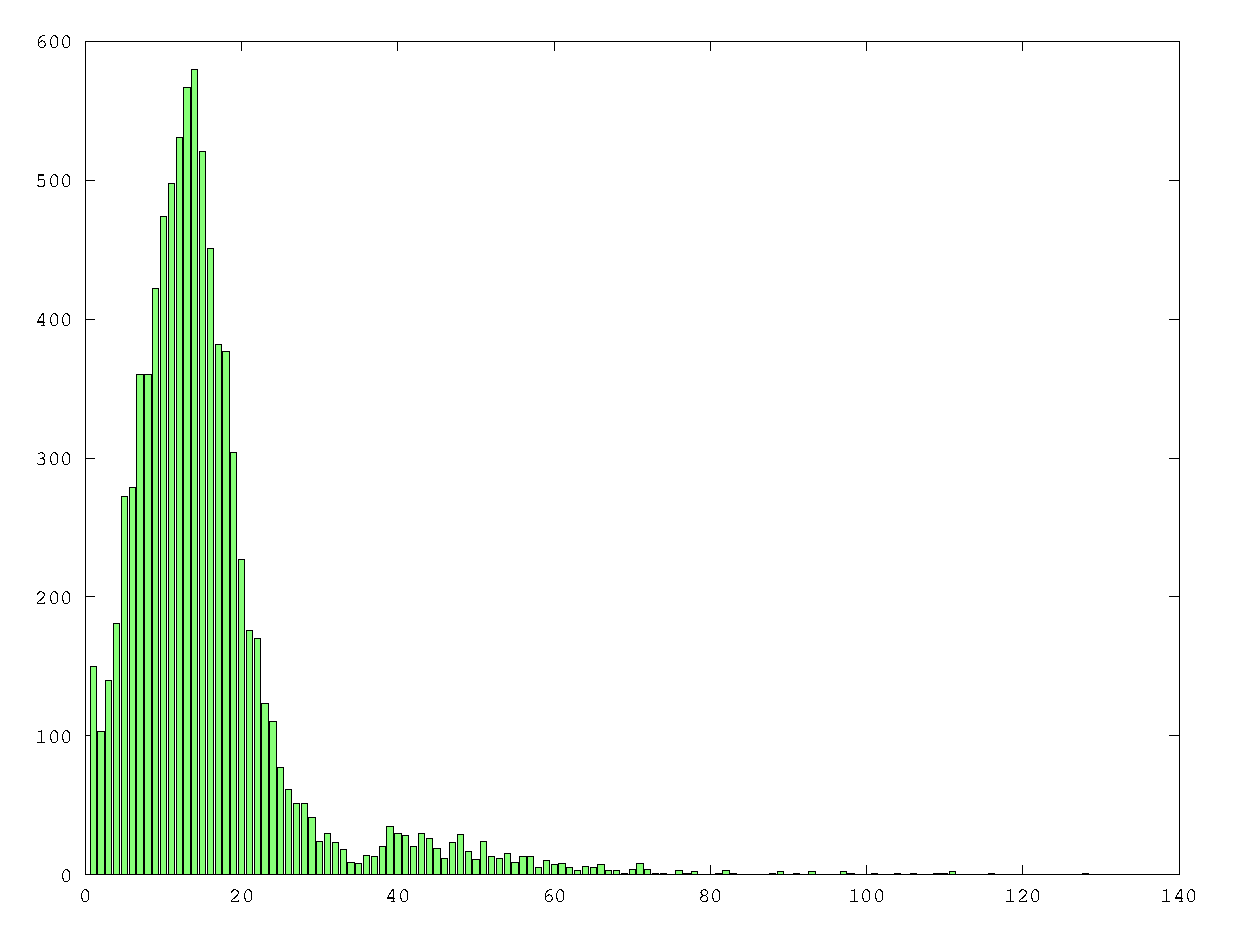
\includegraphics[width=\textwidth]{slike/menisija-polmeri-hist}
    \begin{equation} \resizebox{.3\textwidth}{!}{ $r_{eff} = \sqrt{\frac{A}{\pi}}$} \end{equation}
  \end{column}
\end{columns}
\end{frame}

\begin{frame}{Povprečimo konkavnosti}{Dobimo 'povprečno vrtačo', prilegamo gaussovko na najdene konkavnosti}

\begin{columns}
  \begin{column}{0.5\textwidth}
    \includegraphics[width=\textwidth]{slike/menisija-vrtaca}
    \begin{equation} \resizebox{.75\textwidth}{!}{ $f(r) = A \cdot e^{-\frac{(r-r_0)^2}{\sigma^2}} + C$} \end{equation}
  \end{column}

  \begin{column}{0.45\textwidth}
    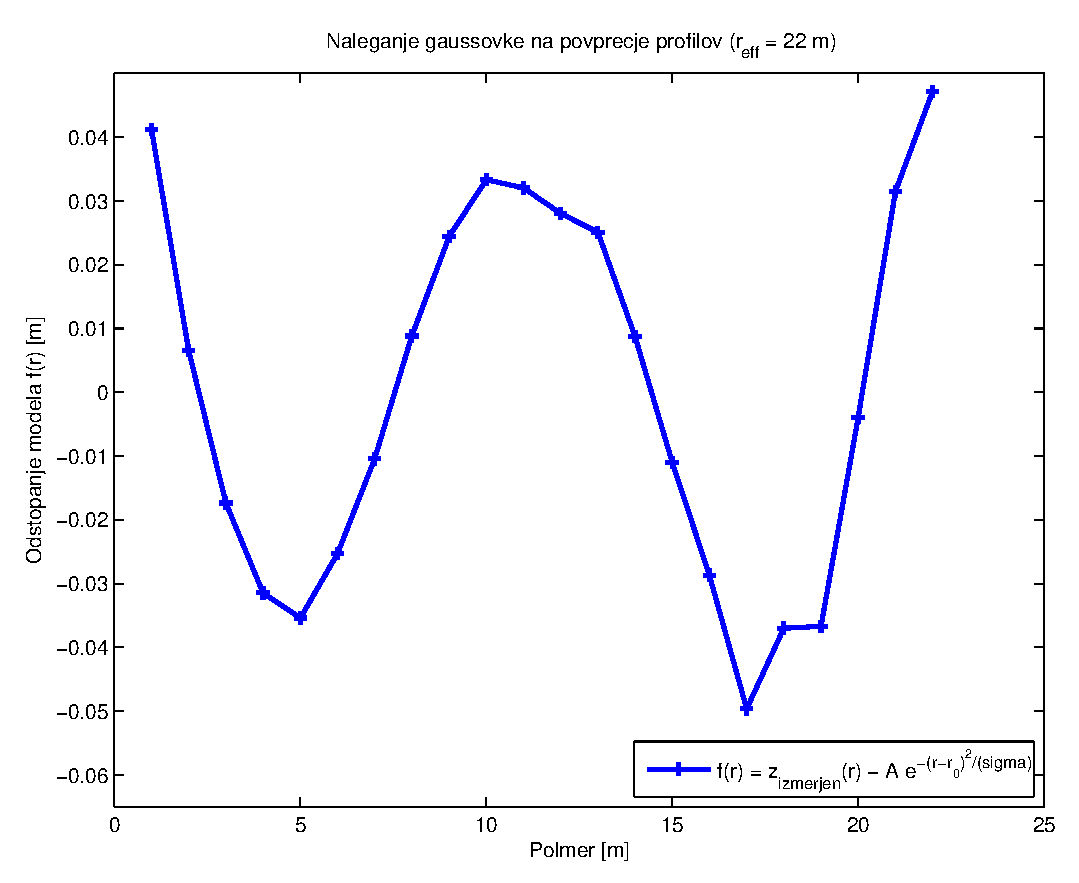
\includegraphics[width=\textwidth]{slike/menisija-profil-21-fit} \\
    \includegraphics[width=\textwidth]{slike/menisija-sigme-hist} \\
    \includegraphics[width=\textwidth]{slike/menisija-globine-hist}
  \end{column}
\end{columns}

\end{frame}


\section{Modeliranje}

\subsection{Kardar-Parisi-Zhang}

\begin{frame}{Kardar-Parisi-Zhang}{}
\end{frame}


\begin{frame}{Blocks}
\begin{block}{Block Title}
You can also highlight sections of your presentation in a block, with it's own title
\end{block}
\begin{theorem}
There are separate environments for theorems, examples, definitions and proofs.
\end{theorem}
\begin{example}
Here is an example of an example block.
\end{example}
\end{frame}


\subsection{Dinamične enačbe}

\begin{frame}{Blocks}
\begin{block}{Block Title}
You can also highlight sections of your presentation in a block, with it's own title
\end{block}
\begin{theorem}
There are separate environments for theorems, examples, definitions and proofs.
\end{theorem}
\begin{example}
Here is an example of an example block.
\end{example}
\end{frame}

\subsection{Difuzijsko dinamične enačbe}

\begin{frame}{Blocks}
\begin{block}{Block Title}
You can also highlight sections of your presentation in a block, with it's own title
\end{block}
\begin{theorem}
There are separate environments for theorems, examples, definitions and proofs.
\end{theorem}
\begin{example}
Here is an example of an example block.
\end{example}
\end{frame}

% Placing a * after \section means it will not show in the
% outline or table of contents.
\section*{Zaključek}

\begin{frame}{Summary}
  \begin{itemize}
  \item
    The \alert{first main message} of your talk in one or two lines.
  \item
    The \alert{second main message} of your talk in one or two lines.
  \item
    Perhaps a \alert{third message}, but not more than that.
  \end{itemize}
  
  \begin{itemize}
  \item
    Outlook
    \begin{itemize}
    \item
      Something you haven't solved.
    \item
      Something else you haven't solved.
    \end{itemize}
  \end{itemize}
\end{frame}



% All of the following is optional and typically not needed. 
\appendix
\section<presentation>*{\appendixname}
\subsection<presentation>*{For Further Reading}

\begin{frame}[allowframebreaks]
  \frametitle<presentation>{For Further Reading}
    
  \begin{thebibliography}{10}
    
  \beamertemplatebookbibitems
  % Start with overview books.

  \bibitem{Author1990}
    A.~Author.
    \newblock {\em Handbook of Everything}.
    \newblock Some Press, 1990.
 
    
  \beamertemplatearticlebibitems
  % Followed by interesting articles. Keep the list short. 

  \bibitem{Someone2000}
    S.~Someone.
    \newblock On this and that.
    \newblock {\em Journal of This and That}, 2(1):50--100,
    2000.
  \end{thebibliography}
\end{frame}

\end{document}


